\section{Setup}
\subsection{Datasets}

We perform experiments on three task-oriented dialog datasets: bAbI Dialog \cite{BordesW16}, CamRest \cite{wenEMNLP2016}, and Stanford Multi-Domain Dataset \cite{Ericsigdial}.

\noindent 
\textbf{bAbI Dialog} consists of synthetically generated dialogs with the goal of restaurant reservation. The dataset consists of five different tasks, all grounded to a KB. This KB is split into two mutually exclusive halves. One half is used to generate the train, validation, and test sets, while the other half is used to create a second test set called the OOV test set. 

\noindent 
\textbf{CamRest} is a human-human dialog dataset, collected using the Wiz-of-Oz framework, also aimed at restaurant reservation. It is typically used to evaluate traditional slot filling systems. In order to make it suitable for end-to-end learning, we stripped the handcrafted state representations and annotations in each dialog, and divided the 676 available dialogs into train, validation, and test sets (406, 135, and 135 dialogs, respectively).

\noindent
\textbf{Stanford Multi-Domain Dataset (SMD)} is another human-human dialog dataset collected using the Wiz-of-Oz framework. Each conversation is between a driver and an in-car assistant. The other datasets consist of dialogs from just one domain (restaurant reservation), whereas SMD consists of dialogs from multiple domains (calendar scheduling, weather information retrieval, and navigation).

\subsection{Knowledge Adaptability (KA) Test Sets}

Each bAbI dialog task has an additional OOV test set, which helps to evaluate a model's robustness to change in information in the KB. A model that perfectly disentangles language and knowledge should have no drop in accuracy on the OOV test set when compared to the non-OOV test set. To measure the degree of disentanglement in a model, we generated 10 additional test sets for each real-world corpus by varying the percentage (in multiples of 10) of unseen entities in the KB. Our adversarial attacks systematically pick random KB entities and replace all their occurrences in the dialog with new entity names. We will refer to these generated dialogs as the \emph{Knowledge Adaptability} (KA) test sets.

\subsection{Baselines}
We compare \sys\ against several existing end-to-end task-oriented dialog systems. These include retrieval models, such as the query reduction network (QRN) \cite{seo2016query}, memory network (MN) \cite{BordesW16}, and gated memory network (GMN) \cite{liu2017gated}. 

We also compare against generative models such as a sequence-to-sequence model (Seq2Seq), a copy augmented Seq2Seq (Seq2Seq+Copy) \cite{ptr-unk}, and Mem2Seq \cite{mem2seq}.\footnote{We thank the authors for releasing a working code at \url{https://github.com/HLTCHKUST/Mem2Seq}} For fairness across models, we do not compare against key-value retrieval networks \cite{Ericsigdial} as they simplify the dataset by canonicalizing all KB words in dialogs.

We noticed that the reported results in the Mem2Seq paper are not directly comparable, as they pre-processed\footnote{Mem2Seq used the following pre-processing on the data: 1) The subject (restaurant name) and object (rating) positions of the rating KB tuples in bAbI dialogs are flipped 2) An extra fact was added to the navigation tasks in SMD which included all the properties (distance, address, etc.) combined together  as the subject and \textit{poi} as the object. See Appendix.} training data in SMD and bAbI datasets. For fair comparisons, we re-run Mem2Seq on the original training datasets. For completeness we mention their reported results (with pre-processing) as Mem2Seq*.

\subsection{Evaluation Metrics}
We evaluate \sys\ and other models based on their ability to generate valid responses. The {\em per-response accuracy} \cite{BordesW16} is the percentage of generated responses that exactly match their respective gold response. The {\em per-dialog accuracy} is the percentage of dialogs with all correctly generated responses. These accuracy metrics are a good measure for evaluating datasets with boilerplate responses such as bAbI. 

To quantify performance on other datasets, we use {\em BLEU} \cite{papineni2002bleu} and {\em Entity F1} \cite{eric2017copy} scores. BLEU measures the overlap of n-grams between the generated response and its gold response and has become a popular measure to compare task-oriented dialog systems. Entity F1 is computed by micro-F1 over KB entities in the entire set of gold responses. 

\subsection{Human Evaluation}
We use two human evaluation experiments to compare (1) the \emph{usefulness} of a generated response with respect to solving the given task, and (2) the \emph{grammatical correctness} and \emph{fluency} of the responses on a 0--3 scale. We obtain human annotations by creating Human Intelligence Tasks (HITs) on Amazon Mechanical Turk (AMT). For each test condition (percentage of unseen entities), we sampled 50 dialogs from Camrest and SMD each, and two AMT workers labeled each system response for both experiments, resulting in 200 labels per condition per dataset per system. We evaluate four systems in this study, leading to a total of 1600 labels per condition. 

% \begin{figure}[t]
%     \centering
%     \subcaptionbox{\label{sfig:testa}}{
%     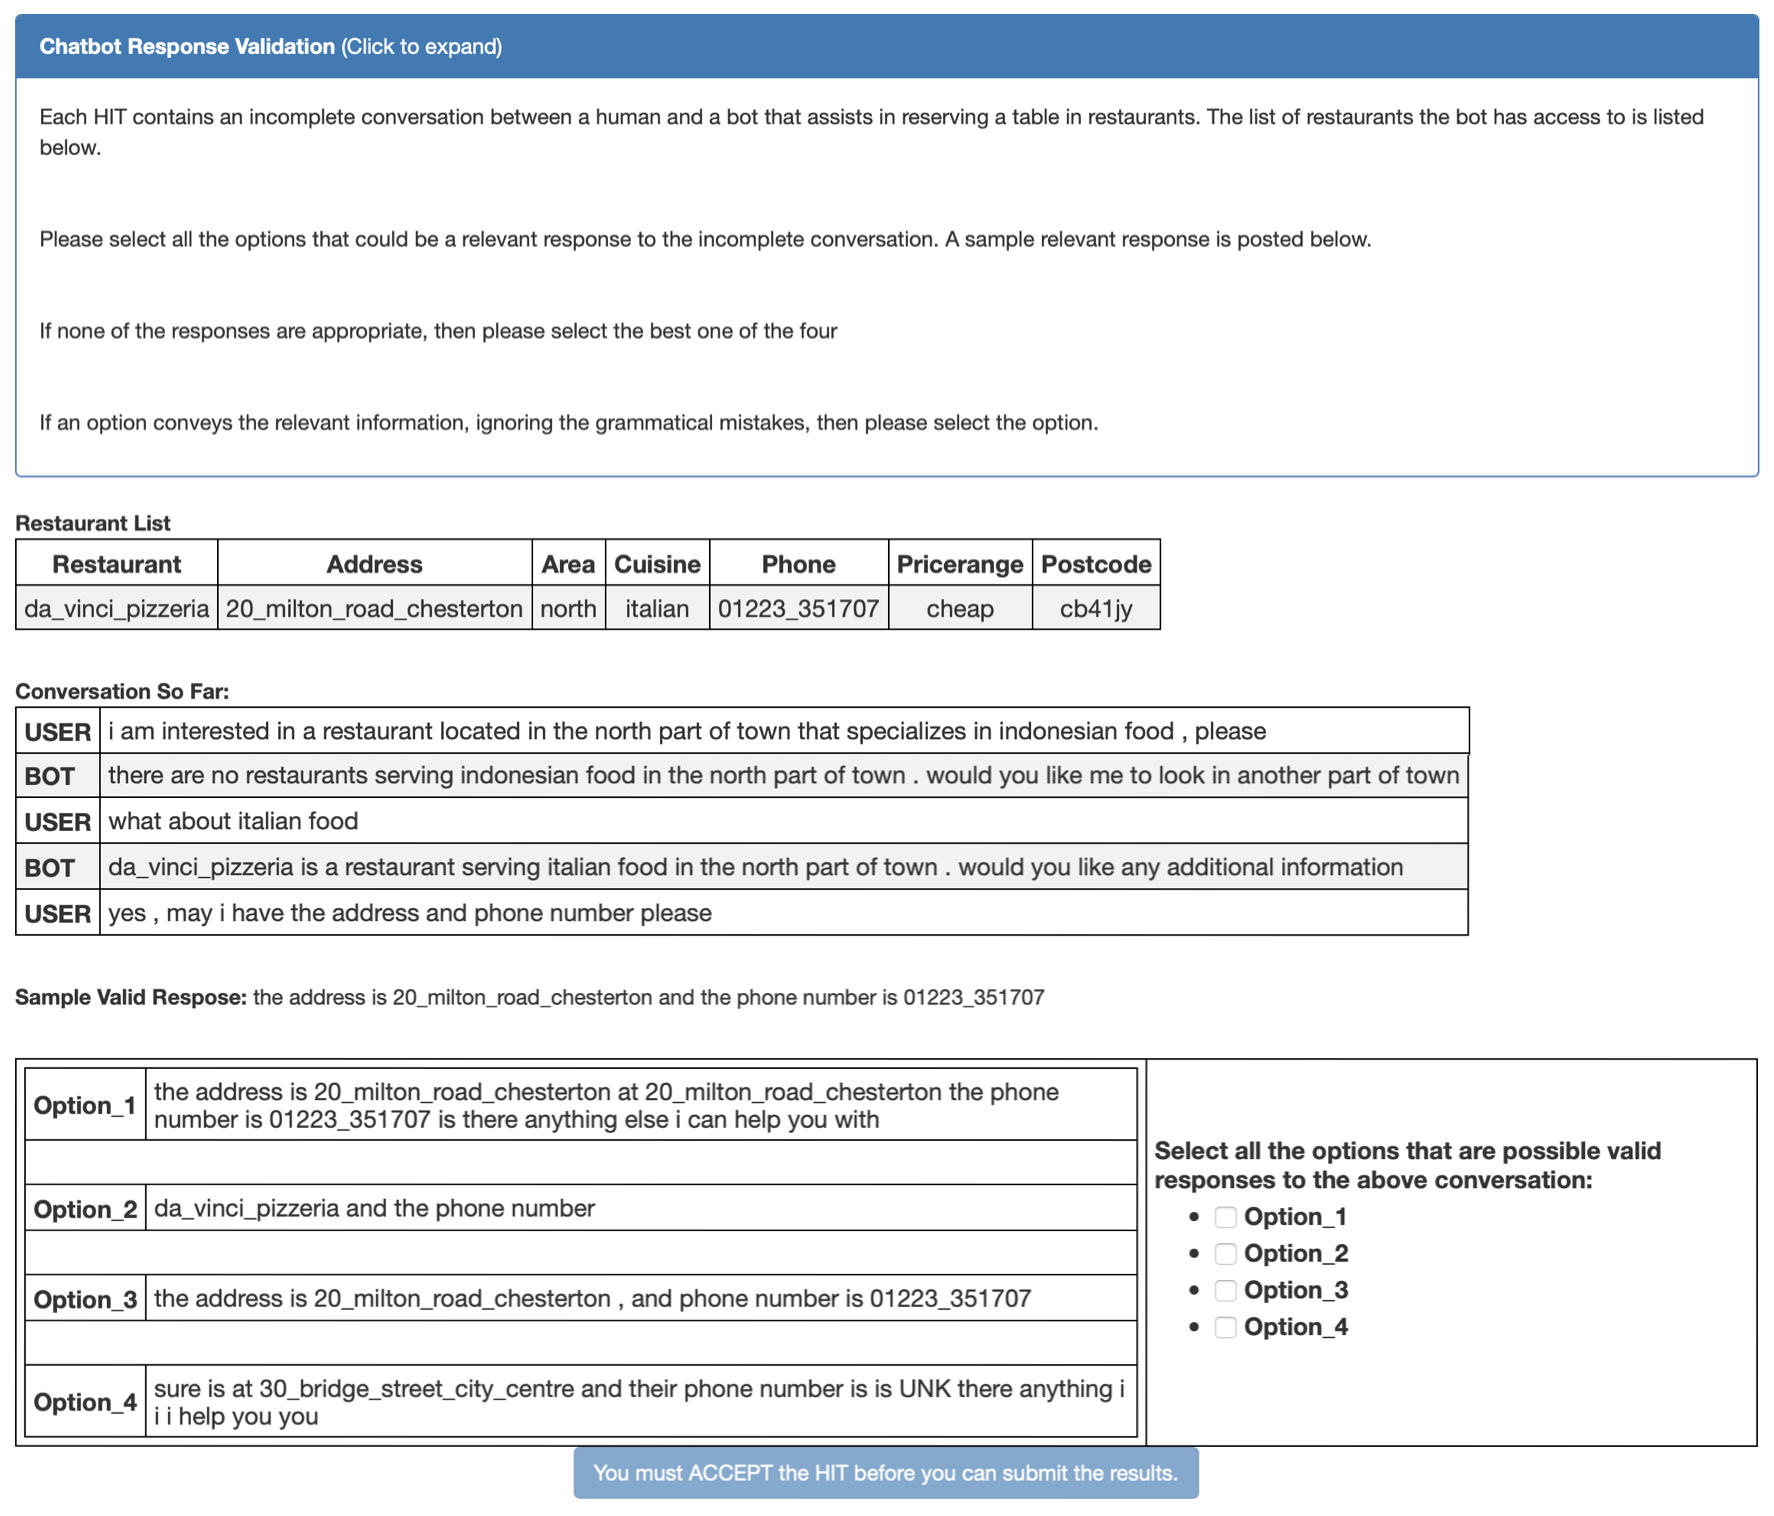
\includegraphics[width=0.8\textwidth]{assets/AMT_screen.png}}
%     \subcaptionbox{\label{sfig:testb}}{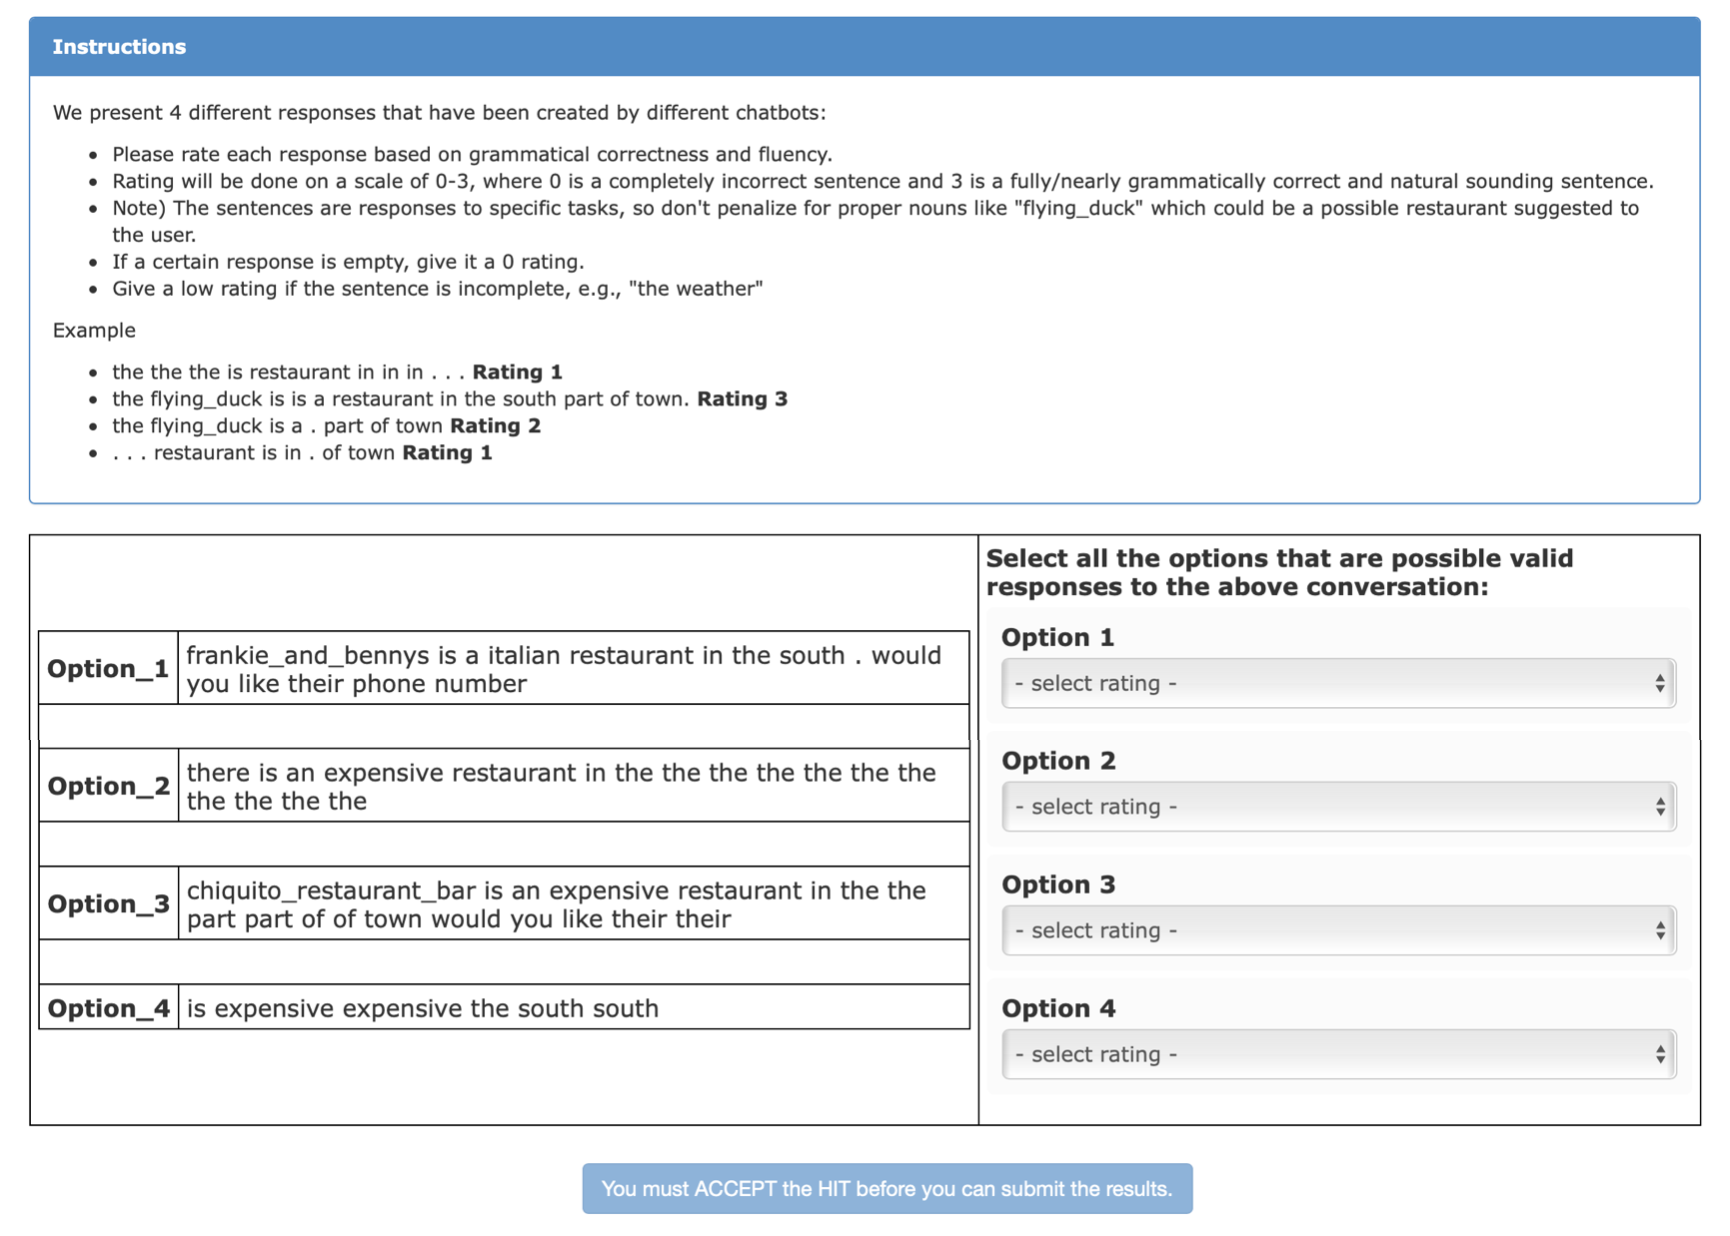
\includegraphics[width=0.9\textwidth]{assets/AMT_screen_grammar.png}}
%     \caption{}
%     \label{fig:amt_rel}
% \end{figure}

\begin{figure}
\centering
\begin{subfigure}{0.8\textwidth}
 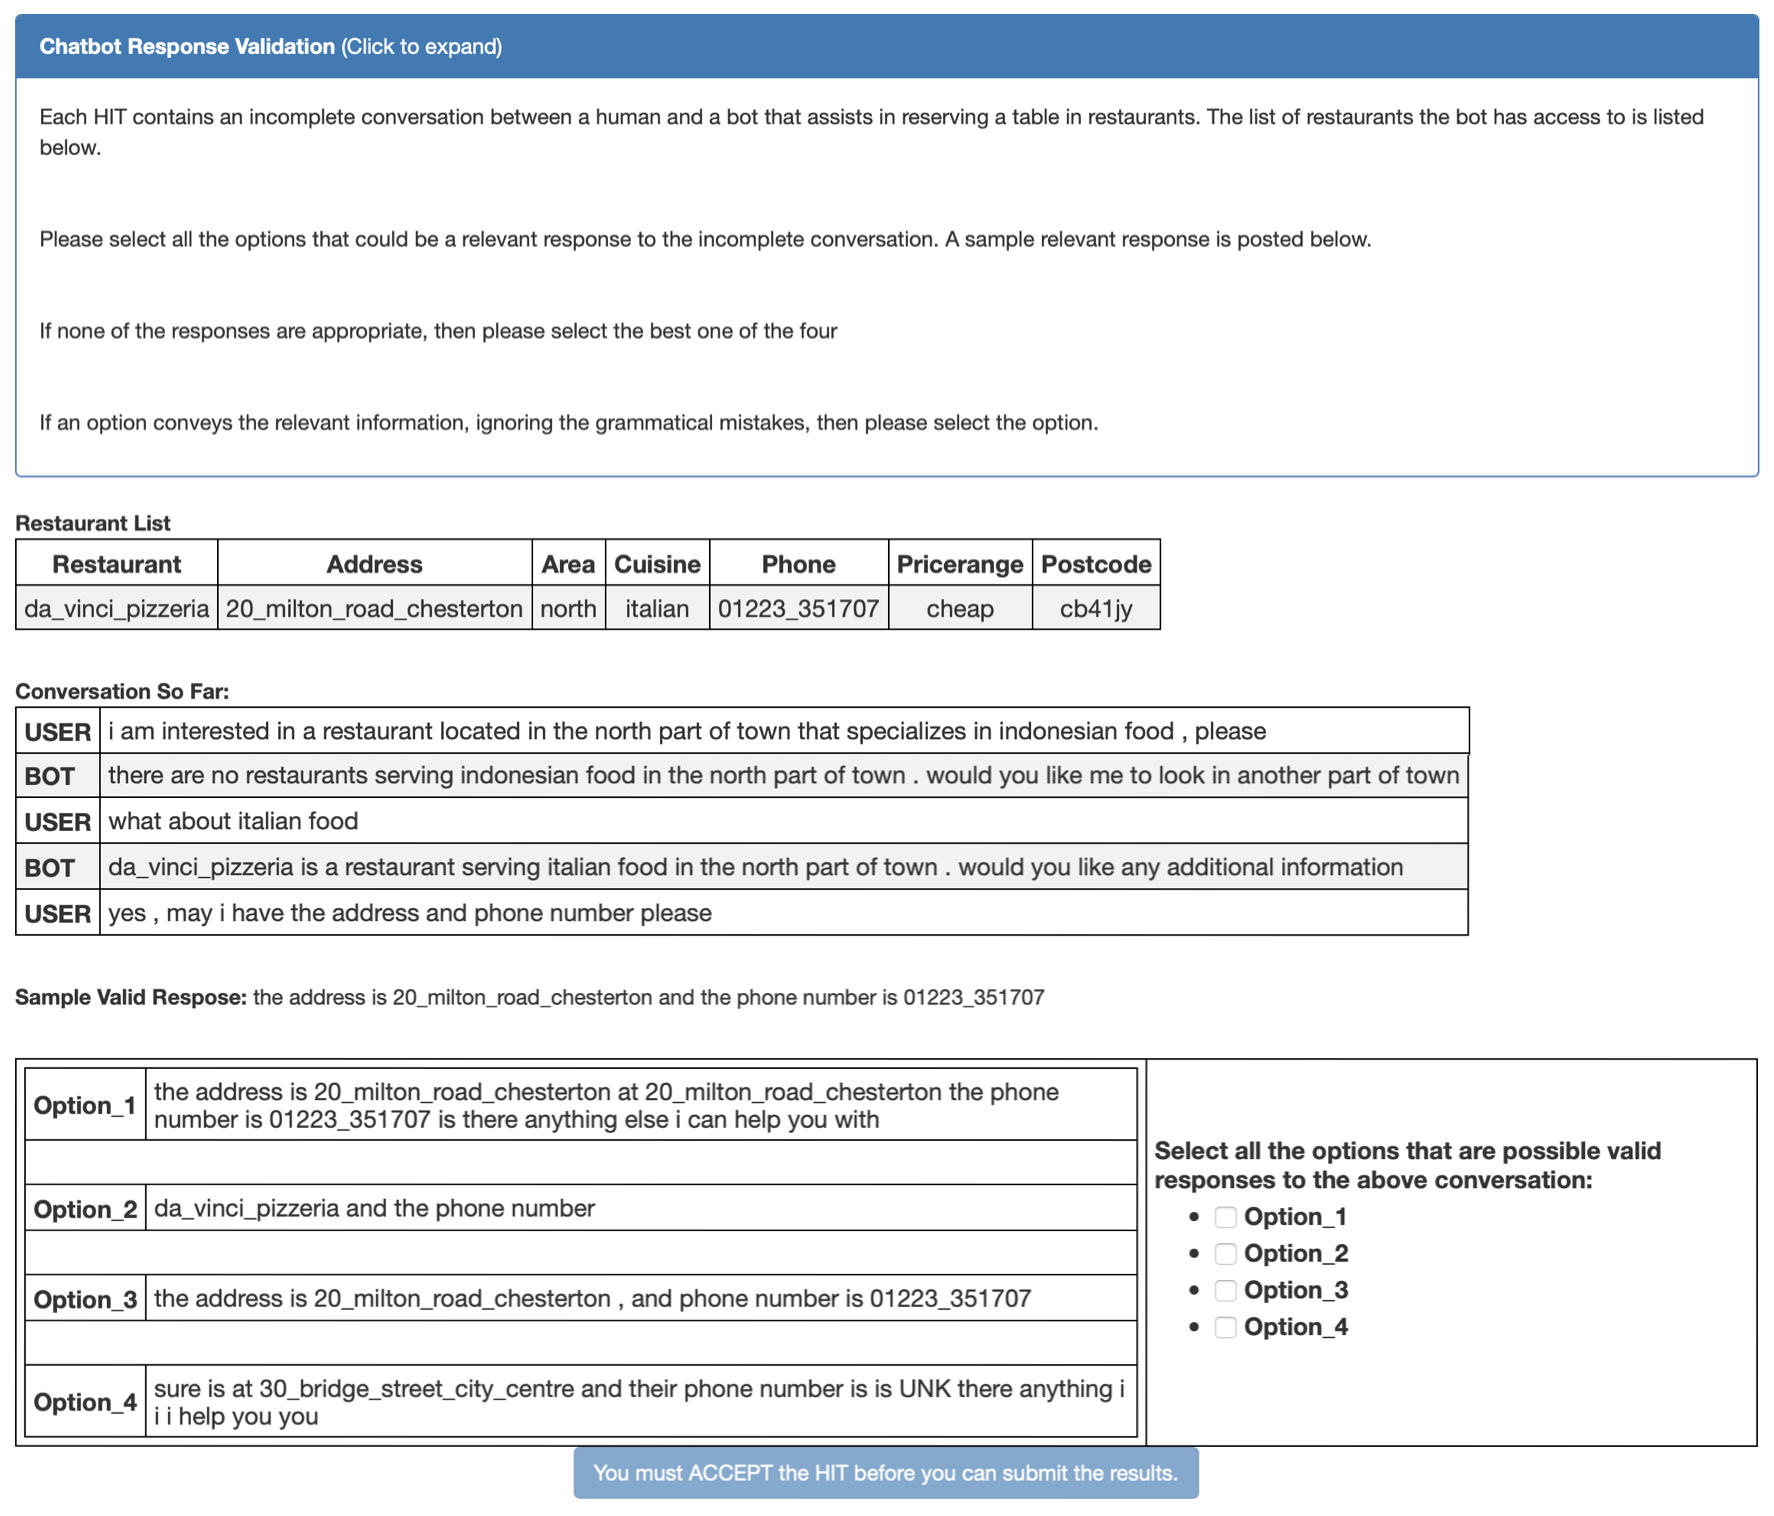
\includegraphics[width=\linewidth]{assets/AMT_screen.png}
 \caption{}\label{fig:testa}
\end{subfigure}

% \vspace*{0.5in}

\begin{subfigure}{0.8\textwidth}
 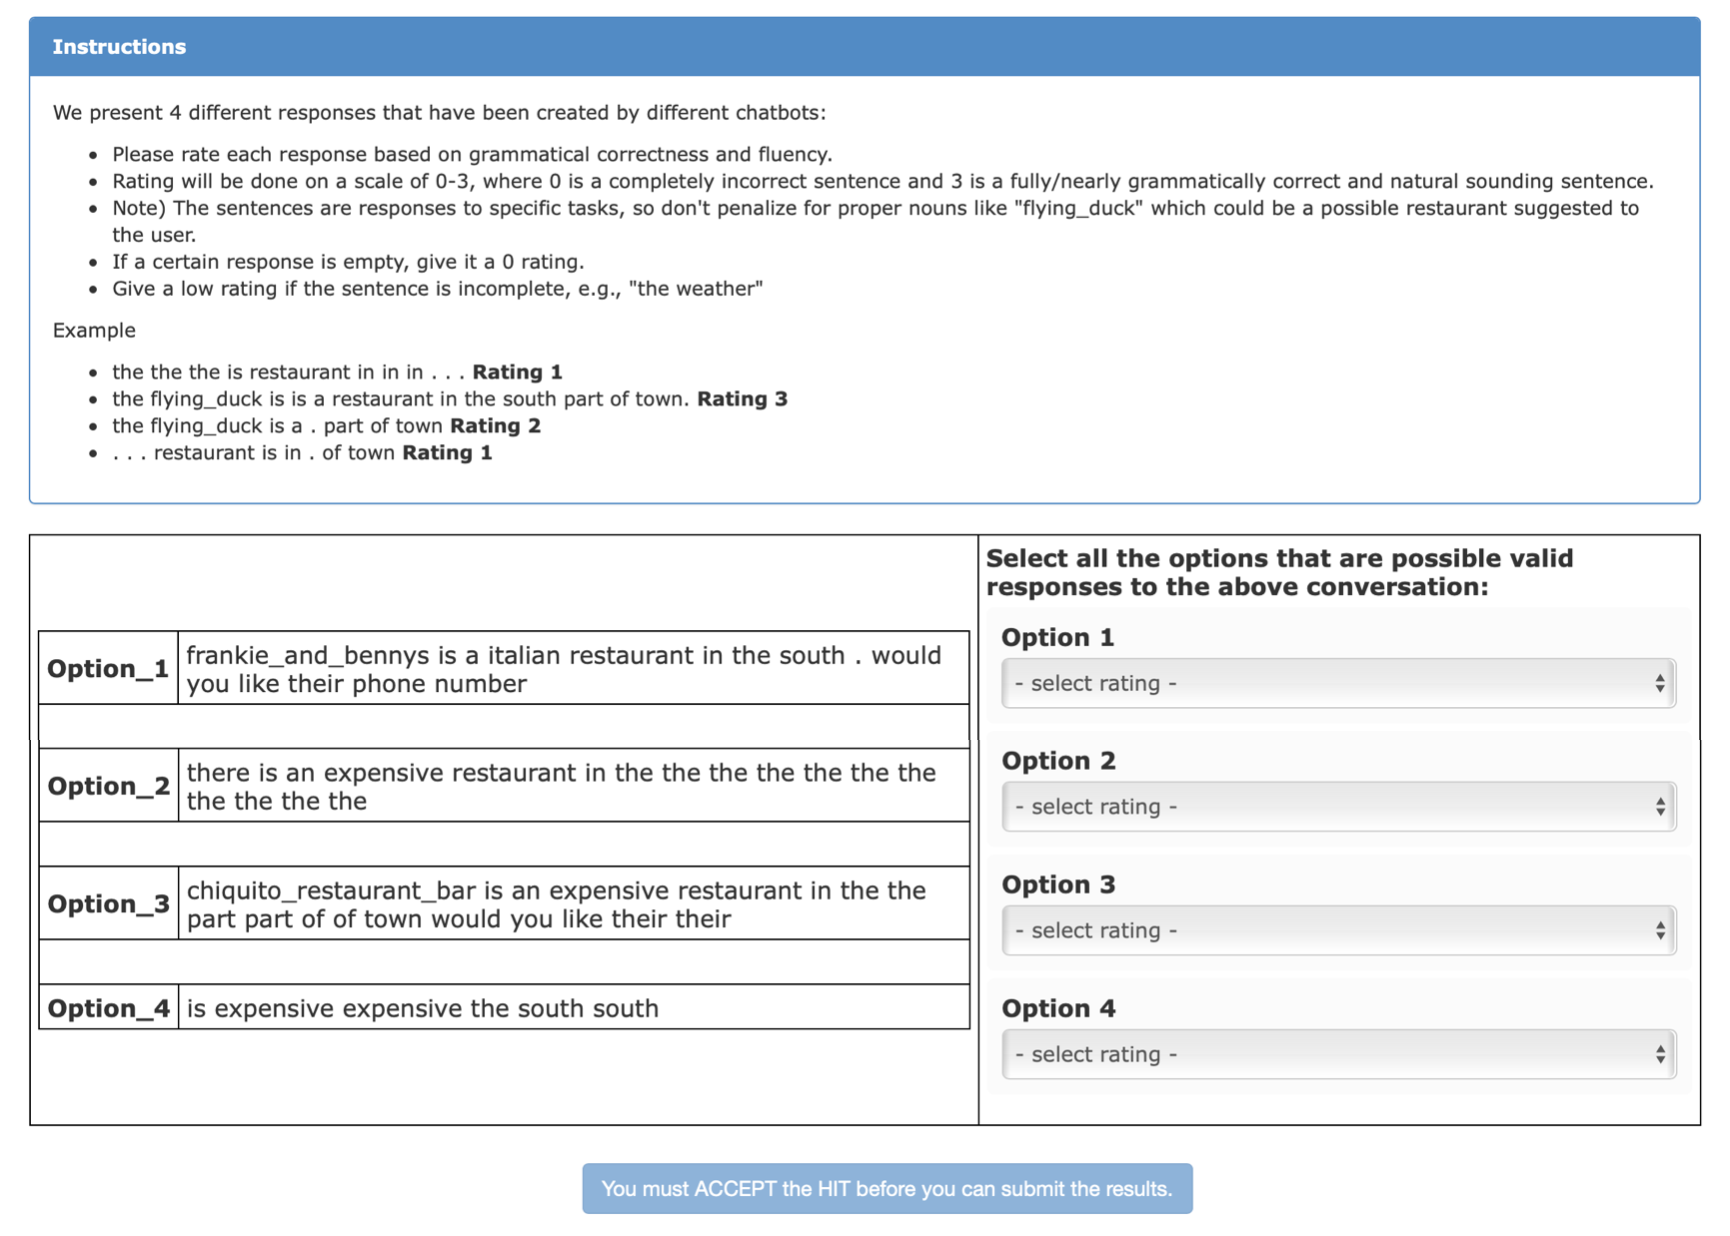
\includegraphics[width=\linewidth]{assets/AMT_screen_grammar.png}
 \caption{}\label{fig:testb}
\end{subfigure}
\caption{A sample HIT on Amazon Mechanical Turk to (a) validate useful responses based on the given dialog context, and (b) validate grammatical correctness of different responses on a scale of 0-3}
\end{figure}

\noindent \textbf{Response Relevance Test} 
We show a sample of an Human Intelligence Task (HIT) on Amazon Mechanical Turk in Figure \ref{fig:testa}. We randomize the responses generated by the three baseline models and \sys\ on the same dialog and ask the user to tick all those response options that seem to capture the relevant information of the given sample response. A total of 200 such annotations were collected for Camrest and SMD each.

\noindent \textbf{Response Grammar Test}
We show a sample of an Human Intelligence Task (HIT) on Amazon Mechanical Turk in Figure \ref{fig:testb}. We randomize the responses generated by the three baseline models and \sys\ on the same dialog and ask the user to rate each response based on the grammatical correctness and natural flow of the sentence. The rating ranges from 0-3 where 0 being the worst and 3 being the best. Note) the sentences were not asked to be rated with respect to each other, but instead as individual occurrences. A total of 200 such annotations were collected for Camrest and SMD each.

\subsection{Training}
We train \sys\ using an Adam optimizer \cite{kingma2014adam} and apply gradient clipping with a clip-value of 40. We identify hyper-parameters based on the evaluation of the held-out validation sets. We sample word embedding, hidden layer, and cell sizes from \{64, 128, 256\} and learning rates from \{10$^{-3}$, 5$\times$10$^{-4}$, 10$^{-4}$\}. The hyper-parameter $\gamma$ in the loss function is chosen between [0-1.5]. The Disentangle Label Dropout rate is sampled from \{0.1, 0.2\}. The number of hops for multi-hop attention in the encoder is sampled from \{1, 3, 6\}. 
We list out the complete set of hyperparameters used to train \sys\ for the various datasets in Table \ref{tab:params}. 

\vspace*{0.5in}

\begin{table*}[ht]
\centering
\footnotesize
\begin{tabular}{c|ccccc}
\toprule
\textbf{Task} & \textbf{Learning Rate} & \textbf{Hops} &  \textbf{Embedding Size} & \textbf{Disentangle Loss Weight} & \textbf{DLD}\\
\midrule
T1 & 0.001 & 1 & 128 & 1.0 & 0.2 \\
T2 & 0.001 & 1 & 128 & 1.0 & 0.2 \\
T3 & 0.0005 & 3 & 128 & 1.5 & 0.2 \\
T4 & 0.001 & 1 & 128 & 1.0 & 0.2 \\
T5 & 0.0005 & 3 & 256 & 1.0 & 0.2 \\
CamRest & 0.0005 & 6 & 256 & 1.0 & 0.2 \\
SMD & 0.0005 & 3 & 256 & 1.0 & 0.1 \\
\bottomrule 
\end{tabular}
\caption{The hyperparameters used to train \sys\ on the different datasets}. 
\label{tab:params}
\end{table*}



